\documentclass{book}

\usepackage{fontspec} % loaded by polyglossia, but included here for transparency
\usepackage{polyglossia}
\setmainlanguage{russian}
\setotherlanguage{english}
% XeLaTeX can use any font installed in your system fonts folder
\newfontfamily\russianfont[Script=Cyrillic]{Ubuntu}
%\newfontfamily\cyrillicfont[Script=Cyrillic]{Ubuntu}

\usepackage{etex}
\usepackage{savesym}
\usepackage{amssymb, amsmath,amsthm,amscd}
%\savesymbol{lrcorner}
\usepackage{txfonts}
\savesymbol{lrcorner}\savesymbol{llcorner}\savesymbol{urcorner}\savesymbol{ulcorner}
%\usepackage{marvosym}
\usepackage{wasysym}
\savesymbol{Sun}\savesymbol{Mercury}\savesymbol{Venus}\savesymbol{Earth}\savesymbol{Mars}\savesymbol{Jupiter}\savesymbol{Saturn}\savesymbol{Uranus}\savesymbol{Neptune}\savesymbol{Pluto}\savesymbol{leftmoon}\savesymbol{rightmoon}\savesymbol{fullmoon}\savesymbol{newmoon}\savesymbol{Aries}\savesymbol{Taurus}\savesymbol{Gemini}\savesymbol{Leo}\savesymbol{Libra}\savesymbol{Scorpio}\savesymbol{diameter}
\usepackage{mathabx}
%\usepackage{stmaryrd}
\usepackage{setspace}
\usepackage{chngcntr}
\usepackage[tt]{titlepic}
\usepackage{enumerate,makecell}
\usepackage{makeidx,tabularx,dashbox}
\usepackage[usenames,dvipsnames]{xcolor}
\usepackage[bookmarks=true,colorlinks=true, linkcolor=MidnightBlue, citecolor=cyan]{hyperref}
\usepackage{lmodern}
\usepackage{graphicx,float}
\usepackage{multirow}
\usepackage{geometry}
\newgeometry{left=1.6in,right=1.6in,top=1.4in,bottom=1.4in}
\restoresymbol{txfonts}{lrcorner}\restoresymbol{txfonts}{llcorner}\restoresymbol{txfonts}{urcorner}\restoresymbol{txfonts}{ulcorner}

\usepackage{color}
\usepackage[all,poly,color,matrix,arrow]{xy}
\makeindex

%\usepackage{showkeys}

\newcommand{\comment}[1]{}

\newcommand{\longnote}[2][4.9in]{\fcolorbox{black}{yellow}{\parbox{#1}{\color{black} #2}}}
\newcommand{\shortnote}[1]{\fcolorbox{black}{yellow}{\color{black} #1}}
\newcommand{\start}[1]{\shortnote{Start here: #1.}}
\newcommand{\q}[1]{\begin{question}#1\end{question}}
\newcommand{\g}[1]{\begin{guess}#1\end{guess}}
\newcommand{\cfbox}[2]{
    \colorlet{currentcolor}{.}
    {\color{#1}
    \fbox{\color{currentcolor}#2}}
}

\def\tn{\textnormal}
\def\mf{\mathfrak}
\def\mc{\mathcal}
\newcommand{\qt}[1]{\tn{``}#1\tn{"}}

\def\ZZ{{\mathbb Z}}
\def\QQ{{\mathbb Q}}
\def\RR{{\mathbb R}}
\def\CC{{\mathbb C}}
\def\AA{{\mathbb A}}
\def\PP{{\mathbb P}}
\def\NN{{\mathbb N}}


\def\Hom{\tn{Hom}}
\def\Path{\tn{Path}}
\def\Paths{\tn{Paths}}
\def\List{\tn{List}}
\def\Aut{\tn{Aut}}
\def\im{\tn{im}}
\def\Fun{\tn{Fun}}
\def\Ob{\tn{Ob}}
\def\Skel{\tn{Skel}}
\def\Op{\tn{Open}}
\def\PK{\tn{PK}}
\def\FK{\tn{FK}}
\def\SEL*{\tn{SEL*}}
\def\Res{\tn{Res}}
\def\hsp{\hspace{.3in}}
\newcommand{\hsps}[1]{{\hspace{2mm} #1\hspace{2mm}}}
\newcommand{\tin}[1]{\text{\tiny #1}}

\def\singleton{\{\smiley\}}
\newcommand{\boxtitle}[1]{\begin{center}#1\end{center}\vspace{-.1in}}
\newcommand{\singlefun}[1]{\star^{#1}}
\newcommand{\pullb}[1]{\Delta_{#1}}
\newcommand{\lpush}[1]{\Sigma_{#1}}
\newcommand{\rpush}[1]{\Pi_{#1}}
\def\lcone{^\triangleleft}
\def\rcone{^\triangleright}
\def\to{\rightarrow}
\def\from{\leftarrow}
\def\down{\downarrrow}
\def\Down{\Downarrow}
\def\taking{\colon}
\def\inj{\hookrightarrow}
\def\surj{\twoheadrightarrow}
\def\too{\longrightarrow}
\newcommand{\xyright}[1]{\xymatrix{~\ar[r]#1&}}
\newcommand{\xydown}[1]{\xymatrix{~\ar[d]#1\\~}}
\newcommand{\xydoown}[1]{\xymatrix{~\ar[ddd]#1\\\parbox{0in}{~}\\\parbox{0in}{~}\\~}}
\def\fromm{\longleftarrow}
\def\tooo{\longlongrightarrow}
\def\tto{\rightrightarrows}
\def\ttto{\equiv\!\!>}
\def\ss{\subseteq}
\def\superset{\supseteq}
\def\iso{\cong}
\def\down{\downarrow}
\def\|{{\;|\;}}
\def\m1{{-1}}
\def\op{^\tn{op}}
\def\loc{\tn{loc}}
\def\la{\langle}
\def\ra{\rangle}
\def\wt{\widetilde}
\def\wh{\widehat}
\def\we{\simeq}
\def\ol{\overline}
\def\ul{\underline}
\def\plpl{+\!\!+\hspace{1pt}}
\def\acts{\lefttorightarrow}
\def\actsRight{\righttoleftarrow}
\def\vect{\overrightarrow}
\def\qeq{\mathop{=}^?}
\def\del{\partial\,}

\def\rr{\raggedright}

%\newcommand{\LMO}[1]{\bullet^{#1}}
%\newcommand{\LTO}[1]{\bullet^{\tn{#1}}}
\newcommand{\LMO}[1]{\stackrel{#1}{\bullet}}
\newcommand{\LTO}[1]{\stackrel{\tt{#1}}{\bullet}}
\newcommand{\LA}[2]{\ar[#1]^-{\tn {#2}}}
\newcommand{\LAL}[2]{\ar[#1]_-{\tn {#2}}}
\newcommand{\obox}[3]{\stackrel{#1}{\fbox{\parbox{#2}{#3}}}}
\newcommand{\labox}[2]{\obox{#1}{1.6in}{#2}}
\newcommand{\mebox}[2]{\obox{#1}{1in}{#2}}
\newcommand{\smbox}[2]{\stackrel{#1}{\fbox{#2}}}
\newcommand{\fakebox}[1]{\tn{$\ulcorner$#1$\urcorner$}}
\newcommand{\sq}[4]{\xymatrix{#1\ar[r]\ar[d]&#2\ar[d]\\#3\ar[r]&#4}}
\newcommand{\namecat}[1]{\begin{center}$#1:=$\end{center}}

\def\monOb{\blacktriangle}

\def\ullimit{\ar@{}[rd]|(.3)*+{\lrcorner}}
\def\urlimit{\ar@{}[ld]|(.3)*+{\llcorner}}
\def\lllimit{\ar@{}[ru]|(.3)*+{\urcorner}}
\def\lrlimit{\ar@{}[lu]|(.3)*+{\ulcorner}}
\def\ulhlimit{\ar@{}[rd]|(.3)*+{\diamond}}
\def\urhlimit{\ar@{}[ld]|(.3)*+{\diamond}}
\def\llhlimit{\ar@{}[ru]|(.3)*+{\diamond}}
\def\lrhlimit{\ar@{}[lu]|(.3)*+{\diamond}}
\newcommand{\clabel}[1]{\ar@{}[rd]|(.5)*+{#1}}
\newcommand{\TriRight}[7]{\xymatrix{#1\ar[dr]_{#2}\ar[rr]^{#3}&&#4\ar[dl]^{#5}\\&#6\ar@{}[u] |{\Longrightarrow}\ar@{}[u]|>>>>{#7}}}
\newcommand{\TriLeft}[7]{\xymatrix{#1\ar[dr]_{#2}\ar[rr]^{#3}&&#4\ar[dl]^{#5}\\&#6\ar@{}[u] |{\Longleftarrow}\ar@{}[u]|>>>>{#7}}}
\newcommand{\TriIso}[7]{\xymatrix{#1\ar[dr]_{#2}\ar[rr]^{#3}&&#4\ar[dl]^{#5}\\&#6\ar@{}[u] |{\Longleftrightarrow}\ar@{}[u]|>>>>{#7}}}


\newcommand{\arr}[1]{\ar@<.5ex>[#1]\ar@<-.5ex>[#1]}
\newcommand{\arrr}[1]{\ar@<.7ex>[#1]\ar@<0ex>[#1]\ar@<-.7ex>[#1]}
\newcommand{\arrrr}[1]{\ar@<.9ex>[#1]\ar@<.3ex>[#1]\ar@<-.3ex>[#1]\ar@<-.9ex>[#1]}
\newcommand{\arrrrr}[1]{\ar@<1ex>[#1]\ar@<.5ex>[#1]\ar[#1]\ar@<-.5ex>[#1]\ar@<-1ex>[#1]}

\newcommand{\To}[1]{\xrightarrow{#1}}
\newcommand{\Too}[1]{\xrightarrow{\ \ #1\ \ }}
\newcommand{\From}[1]{\xleftarrow{#1}}
\newcommand{\Fromm}[1]{\xleftarrow{\ \ #1\ \ }}

\newcommand{\Adjoint}[4]{\xymatrix@1{#2 \ar@<.5ex>[r]^-{#1} & #3 \ar@<.5ex>[l]^-{#4}}}
\newcommand{\adjoint}[4]{\xymatrix{#1\taking #2\ar@<.5ex>[r]& #3\hspace{1pt}:\hspace{-2pt} #4\ar@<.5ex>[l]}}

\newcommand{\prodmap}[2]{\la#1,#2\ra}
\newcommand{\pb}[3]{\prodmap{#1}{#1}_{#3}}
\newcommand{\coprodmap}[2]{{\left\{\parbox{.1in}{#1\\#2}\right.}}
\newcommand{\po}[3]{\coprodmap{#1}{#2}}

\def\id{\tn{id}}
\def\ids{\tn{ids}}
\def\Top{{\bf Top}}
\def\Cat{{\bf Cat}}
\def\Oprd{{\bf Oprd}}
\def\Str{{\bf Str}}
\def\Mon{{\bf Mon}}
\def\Grp{{\bf Grp}}
\def\Grph{{\bf Grph}}
\def\Type{{\bf Type}}
\def\Supp{{\bf Supp}}
\def\Dist{{\bf Dist}}
\def\Vect{{\bf Vect}}
\def\Kls{{\bf Kls}}
\def\Prop{{\bf Prop}}
\def\FLin{{\bf FLin}}
\def\Set{{\bf Set}}
\def\Sets{{\bf Sets}}
\def\PrO{{\bf PrO}}
\def\Star{{\bf Star}}
\def\Cob{{\bf Cob}}
\def\Qry{{\bf Qry}}
\def\set{{\text \textendash}{\bf Set}}
\def\sSet{{\bf sSet}}
\def\sSets{{\bf sSets}}
\def\Grpd{{\bf Grpd}}
\def\Pre{{\bf Pre}}
\def\Shv{{\bf Shv}}
\def\Rings{{\bf Rings}}
\def\bD{{\bf \Delta}}
\def\dispInt{\parbox{.1in}{$\int$}}
\def\bhline{\Xhline{2\arrayrulewidth}}
\def\bbhline{\Xhline{2.5\arrayrulewidth}}
\def\bbbhline{\Xhline{3\arrayrulewidth}}


\def\colim{\mathop{\tn{colim}}}
\def\hocolim{\mathop{\tn{hocolim}}}

\def\mcA{\mc{A}}
\def\mcB{\mc{B}}
\def\mcC{\mc{C}}
\def\mcD{\mc{D}}
\def\mcE{\mc{E}}
\def\mcF{\mc{F}}
\def\mcG{\mc{G}}
\def\mcH{\mc{H}}
\def\mcI{\mc{I}}
\def\mcJ{\mc{J}}
\def\mcK{\mc{K}}
\def\mcL{\mc{L}}
\def\mcM{\mc{M}}
\def\mcN{\mc{N}}
\def\mcO{\mc{O}}
\def\mcP{\mc{P}}
\def\mcQ{\mc{Q}}
\def\mcR{\mc{R}}
\def\mcS{\mc{S}}
\def\mcT{\mc{T}}
\def\mcU{\mc{U}}
\def\mcV{\mc{V}}
\def\mcW{\mc{W}}
\def\mcX{\mc{X}}
\def\mcY{\mc{Y}}
\def\mcZ{\mc{Z}}

\def\undsc{\rule{2mm}{0.4pt}}
\def\Loop{{\mcL oop}}
\def\LoopSchema{{\parbox{.5in}{\fbox{\xymatrix{\LMO{s}\ar@(l,u)[]^f}}}}}

\newtheorem{theorem}[subsubsection]{Theorem}
\newtheorem{lemma}[subsubsection]{Lemma}
\newtheorem{proposition}[subsubsection]{Proposition}
\newtheorem{corollary}[subsubsection]{Corollary}
\newtheorem{fact}[subsubsection]{Fact}

\theoremstyle{remark}
\newtheorem{remark}[subsubsection]{Remark}
\newtheorem{example}[subsubsection]{Example}
\newtheorem{warning}[subsubsection]{Warning}
\newtheorem{question}[subsubsection]{Question}
\newtheorem{guess}[subsubsection]{Guess}
\newtheorem{answer}[subsubsection]{Answer}
\newtheorem{construction}[subsubsection]{Construction}
\newtheorem{rules}[subsubsection]{Rules of good practice}
\newtheorem{exc}[subsubsection]{Exercise}
\newenvironment{exercise}{\begin{exc}}{\hspace*{\fill}$\lozenge$\end{exc}}
\newtheorem{app}[subsubsection]{Application}
\newenvironment{application}{\begin{app}}{\hspace*{\fill}$\lozenge\lozenge$\end{app}}

%\newenvironment{exercise}{\addtocounter{theorem}{1}\vspace{.1in}\begin{sloppypar}\noindent{\em Exercise}\;\arabic{chapter}.\arabic{section}.\arabic{subsection}.\arabic{theorem}.}{\end{sloppypar}\vspace{.1in}}

\newenvironment{slogan}{\addtocounter{subsubsection}{1}\vspace{.1in}\begin{sloppypar}\noindent{\em Slogan}\;\arabic{chapter}.\arabic{section}.\arabic{subsection}.\arabic{subsubsection}. \begin{quote}``\slshape}{"\end{quote}\end{sloppypar}\vspace{.1in}}

%\newenvironment{application}{\addtocounter{subsubsection}{1}\vspace{.1in}\begin{sloppypar}\noindent{\em Application}\;\arabic{chapter}.\arabic{section}.\arabic{subsection}.\arabic{subsubsection}. \begin{quote}}{\end{quote}\end{sloppypar}\vspace{.1in}}
\makeatletter\let\c@figure\c@equation\makeatother%Aligns figure numbering and equation numbering.

\theoremstyle{definition}
\newtheorem{definition}[subsubsection]{Definition}
\newtheorem{notation}[subsubsection]{Notation}
\newtheorem{conjecture}[subsubsection]{Conjecture}
\newtheorem{postulate}[subsubsection]{Postulate}


%\newtheorem{theorem}{Theorem}[subsection]
%\newtheorem{lemma}[theorem]{Lemma}
%\newtheorem{proposition}[theorem]{Proposition}
%\newtheorem{corollary}[theorem]{Corollary}
%\newtheorem{fact}[theorem]{Fact}
%
%\theoremstyle{remark}
%\newtheorem{remark}[theorem]{Remark}
%\newtheorem{example}[theorem]{Example}
%\newtheorem{warning}[theorem]{Warning}
%\newtheorem{question}[theorem]{Question}
%\newtheorem{guess}[theorem]{Guess}
%\newtheorem{answer}[theorem]{Answer}
%\newtheorem{construction}[theorem]{Construction}
%\newtheorem{rules}[theorem]{Rules of good practice}
%\newtheorem{exc}[theorem]{Exercise}
%%\newenvironment{exercise}{\addtocounter{theorem}{1}\vspace{.1in}\begin{sloppypar}\noindent{\em Exercise}\;\arabic{chapter}.\arabic{section}.\arabic{subsection}.\arabic{theorem}.}{\end{sloppypar}\vspace{.1in}}
%\newenvironment{exercise}{\begin{exc}}{\hspace*{\fill}$\lozenge$\end{exc}}
%
%\theoremstyle{definition}
%\newtheorem{definition}[theorem]{Definition}
%\newtheorem{notation}[theorem]{Notation}
%\newtheorem{conjecture}[theorem]{Conjecture}
%\newtheorem{postulate}[theorem]{Postulate}

\def\Finm{{\bf Fin_{m}}}
\def\Prb{{\bf Prb}}
\def\Prbs{{\wt{\bf Prb}}}
\def\El{{\bf El}}
\def\Gr{{\bf Gr}}
\def\DT{{\bf DT}}
\def\DB{{\bf DB}}
\def\Tables{{\bf Tables}}
\def\Sch{{\bf Sch}}
\def\Fin{{\bf Fin}}
\def\P{{\bf P}}
\def\SC{{\bf SC}}
\def\ND{{\bf ND}}
\def\Poset{{\bf Poset}}


\newcommand{\MainCatLarge}[1]{
	\stackrel{#1}{
		\parbox{4.5in}{\fbox{\parbox{4.4in}{\begin{center}\underline{{\tt Employee} manager worksIn $\simeq$ {\tt Employee} worksIn}\hsp  \underline{{\tt Department} secretary worksIn $\simeq$ {\tt Department}}\end{center}~\\\\\\
			\xymatrix@=8pt{&\LTO{Employee}\ar@<.5ex>[rrrrr]^{\tn{worksIn}}\ar@(l,u)[]+<5pt,10pt>^{\tn{manager}}\ar[dddl]_{\tn{first}}\ar[dddr]^{\tn{last}}&&&&&\LTO{Department}\ar@<.5ex>[lllll]^{\tn{secretary}}\ar[ddd]^{\tn{name}}\\\\\\\LTO{FirstNameString}&&\LTO{LastNameString}&~&~&~&\LTO{DepartmentNameString}
			}
		}}}
	}
}
\def\GrIn{{\bf GrIn}}
\def\GrInSchema{\xymatrix{\LMO{Ar}\ar@<.5ex>[r]^{src}\ar@<-.5ex>[r]_{tgt}&\LMO{V\!e}}}
%\CompileMatrices
%\pdfoutput=1

\setcounter{secnumdepth}{3}
\setcounter{tocdepth}{1}

\def\sub{\begin{itemize}\item}
\def\sexc{\begin{enumerate}[a.)]\setlength{\itemsep}{.1cm}\setlength{\parskip}{.1cm}\item}
\def\next{\item}
\def\endsub{\end{itemize}}
\def\endsexc{\end{enumerate}}

%%%%%

\begin{document}
\begin{english}

\title{
  ~\\Category Theory for Scientists\\
  \begin{russian}Теория категорий для науки\end{russian}
}
\author{
  David I. Spivak\\
  \begin{russian}Давид И. Спивак\end{russian}
}
\titlepic{\vspace{1.3in}\dashbox{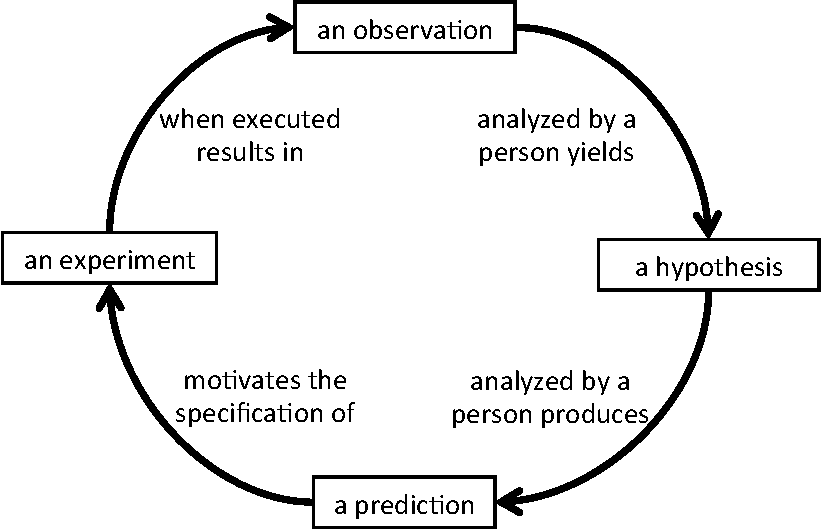
\includegraphics[width=.8\textwidth]{ScientificMethod}}\\\vspace{.3in}\Large How can mathematics make this diagram meaningful?%What does this diagram intend to communicate?
\normalsize}
\maketitle

\chapter*{Preface / \begin{russian}Предисловие\end{russian}}

An early version of this book was put on line in February 2013 to serve as the textbook for my course \href{http://math.mit.edu/~dspivak/teaching/sp13/}{\text Category Theory for Scientists} taught in the spring semester of 2013 at MIT. During that semester, students provided me with hundreds of comments and questions, which led to a substantial improvement (and the addition of 50 pages) to the original document.

\begin{russian}Ранняя версия данной книги была представлена в феврале 2013 в качестве учебника для моего курса \href{http://math.mit.edu/~dspivak/teaching/sp13/}{\text Теория категорий для ученых}, который читался в весеннем семестре 2013 в MIT. В течение семестра студенты передали мне сотни комментариев и вопросов, которые привели к существенному улучшению исходного текста (и к добавлению 50 страниц).\end{russian}

In the summer of 2013 I signed a contract with the MIT Press to publish a new version of this work under the title {\em Category Theory for the Sciences}. Because I am committed to the open source development model I insisted that a version of this book, namely the one you are reading, remain freely available online. The MIT Press version will of course not be free.

\begin{russian}Летом 2013 я подписал контракт с MIT Press о публикации новой версии данной работы под заглавием {\em Теория категорий для наук}. Поскольку я являюсь приверженцем подхода открытого исходного кода, я настоял на том, что отдельная версия этой книги, а именно --- та, которую вы сейчас читаете, останется доступной бесплатно онлайн. \end{russian}

Other than the title, there are two main differences between the present version and the MIT Press version. The first difference is that I will do a full edit with the help of professional editors from the Press. The second difference is that I will write up solutions to the book's (approximately 280) exercises; some of these will be included in the published version, whereas the rest will be available by way of a password-protected page, accessible only to professors who teach the subject.

\begin{russian}Помимо заголовка, есть еще два основных различия данной версии и версии MIT Press. Первое различие состоит в том, что я проведу кардинальное редактирование при помощи профессиональных редакторов. Второе различие --- в том, что я напишу решения для упражнений этой книги (приблизительно 280); некоторые из них будут включены в опубликованную версию, тогда как остальные будут размещены на защищенной паролем странице, доступные только преподавателям, ведущим данный предмет. \end{russian}

\tableofcontents

%%%%%%%% Chapter %%%%%%%%

\chapter{Introduction / Введение}

The title page of this book contains a graphic that we reproduce here.\\
\begin{russian}Титульная страница данной книги содержит рисунок, который мы воспроизводим ниже.\end{russian}
\begin{align}\label{dia:scientific method}
\dashbox{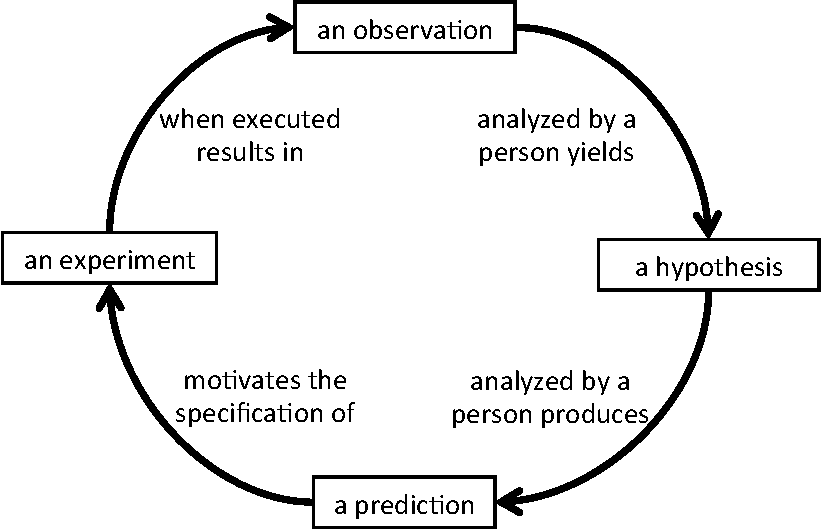
\includegraphics[width=.7\textwidth]{ScientificMethod}}
\end{align}
It is intended to evoke thoughts of the scientific method.\\
\begin{russian}Он призван наводить на мысли о научном методе.\end{russian} \begin{quote}
A hypothesis analyzed by a person produces a prediction, which motivates the specification of an experiment, which when executed results in an observation, which analyzed by a person yields a hypothesis.

\begin{russian}Гипотеза, выведенная человеком, приводит к предсказанию, которое мотивирует описание эксперимента, который, после выполнения, приводит к наблюдениям, которые, будучи проанализированы человеком, приводят к гипотезе.\end{russian}
\end{quote}
This sounds valid, and a good graphic can be exceptionally useful for leading a reader through the story that the author wishes to tell. \\
\begin{russian}Это похоже на истину; кроме того, хорошая картинка может быть исключительно полезна, чтобы провести читателя сквозь историю, которую автор желает поведать.\end{russian}

Interestingly, a graphic has the power to evoke feelings of understanding, without really meaning much. The same is true for text: it is possible to use a language such as English to express ideas that are never made rigorous or clear. When someone says ``I believe in free will," what does she believe in? We may all have some concept of what she's saying---something we can conceptually work with and discuss or argue about. But to what extent are we all discussing the same thing, the thing she intended to convey?

\begin{russian}Любопытный факт: картинка имеет способность вызывать ощущение понимания, не неся при этом особого смысла. То же верно и для слов: язык вроде английского способен выражать идеи, которые в принципе невозможно сделать строгими или ясными. Если некто заявляет "Я верю в свободу воли," то во что некто верит? Все мы можем иметь некоторые представления о том, что этот некто говорит --- такие, с которыми можно концептуально работать, рассуждать, аргументировать. Но до какой степени мы все будем обсуждать одну и ту же вещь, --- вещь, которую некто собирался сообщить? \end{russian}

Science is about agreement. When we supply a convincing argument, the result of this convincing is agreement. When, in an experiment, the observation matches the hypothesis---success!---that is agreement. When my methods make sense to you, that is agreement. When practice does not agree with theory, that is disagreement. Agreement is the good stuff in science; it's the high fives.

\begin{russian} Суть науки --- в согласии. Когда мы предлагаем убедительный аргумент,  результатом этой убедительности является согласие. Когда в ходе эксперимента наблюдения совпадают с гипотезой, --- вот удача! --- это согласие. Когда мои методы имеют смысл и для вас, это согласие. Когда же практика не соответствует теории, это несогласие. Согласие --- вот лучшая материя в науке; оно подобно рукопожатию. \end{russian}

But it is easy to think we're in agreement, when really we're not. Modeling our thoughts on heuristics and pictures may be convenient for quick travel down the road, but we're liable to miss our turnoff at the first mile. The danger is in mistaking our convenient conceptualizations for what's actually there. It is imperative that we have the ability at any time to ground out in reality. What does that mean?

\begin{russian} Однако легко попасть в ситуацию, когда мы думаем, будто согласны, но на самом деле это не так. Моделирования наших размышлений в эвристиках или картинках может быть удобно для быстрого движения напрямик, но нам самим придется нести ответственность, если мы пропустим нужный поворот на первой же миле. Опасность --- в ошибочном выборе слишком удобной концептуализации для того, что происходит в на самом деле. В любой момент необходимо иметь возможность привязаться к реальности. Что это означает? \end{russian}

Data. Hard evidence. The physical world. It is here that science touches down and heuristics evaporate. So let's look again at the diagram on the cover. It is intended to evoke an idea of how science is performed. Is there hard evidence and data to back this theory up? Can we set up an experiment to find out whether science is actually performed according to such a protocol? To do so we have to shake off the stupor evoked by the diagram and ask the question: ``what does this diagram intend to communicate?"

\begin{russian} Данные. Железные подтверждения. Физический мир. Именно здесь наука приземляется, и испаряются эвристики. Так что давайте взглянем на диаграмму на обложке еще раз. Она предназначена вызывать идею о том, как делают науку. Но имеются ли железные подтверждения и данные, стоящие за подобной теорией? Способны ли мы организовать эксперимент для проверки того, что науку делают именно в соответствии с подобным протоколом? Чтобы сделать это, мы должны сбросить ступор, вызванный диаграммой, и задаться вопросом: "Что эта диаграмма должна нам сообщать?" \end{russian}

In this course I will use a mathematical tool called {\em ologs}, or ontology logs, to give some structure to the kinds of ideas that are often communicated in pictures like the one on the cover. Each olog inherently offers a framework in which to record data about the subject. More precisely it encompasses a {\em database schema}, which means a system of interconnected tables that are initially empty but into which data can be entered. For example consider the olog below\\
\begin{russian}В этом курсе я буду использовать математический инструмент, называемый {\em ологами} или же онтологическими записями, чтобы придать некую структуру тем видам идей, о которых зачастую сообщается в картинках, подобных той, что изображена на обложке. Каждый олог по своей сути представляет собой конструкцию, в которой записаны данные о предмете обсуждения. Более точно, они отражают {\em схему базы данных}, что означает систему взаимосвязанных таблиц, которые вначале пусты, но в которые могут быть внесены данные. Для примера рассмотрим такой олог \end{russian}
$$\xymatrix{
\obox{}{.5in}{\begin{russian}масса\end{russian}}&&\obox{}{1.1in}{\begin{russian}объект массы \end{russian}$m$ \begin{russian}удерживаемый на высоте \end{russian}$h$ \begin{russian}над землей\end{russian}}\LAL{ll}{\footnotesize\begin{russian}имеет массу\end{russian}}\LA{rrdd}{\hspace{.4in}\parbox{1in}{\singlespace \footnotesize \begin{russian}при падении требуется определенное число секунд до ударения о землю\end{russian}}}\LAL{dd}{\parbox{.7in}{\singlespace\footnotesize\begin{russian}имеет высоту в метрах\end{russian}}}&&\\\\
&&\obox{}{1in}{\begin{russian}действительное число \end{russian} $h$}\ar@{}[uurr]|(.35){?}\ar[rr]_-{\sqrt{2h\div 9.8}}&\hspace{.3in}&\obox{}{.9in}{\begin{russian}действительное число \end{russian} }
}
$$
This olog represents a framework in which to record data about objects held above the ground, their mass, their height, and a comparison (the ?-mark in the middle) between the number of seconds till they hit the ground and a certain real-valued function of their height. We will discuss ologs in detail throughout this course.\\
\begin{russian}Данный олог представляет собой конструкцию, в которой для объектов, находящихся над поверхностью земли, записаны: их масса, их высота и соответствие (значок ? в середине) между числом секунд, за которое они достигают земли, с определенной действительнозначной функцией их высоты. Ологи мы детально обсудим по ходу этого курса. \end{russian}

The picture in (\ref{dia:scientific method}) looks like an olog, but it does not conform to the rules that we lay out for ologs in Section \ref{sec:ologs}. In an olog, every arrow is intended to represent a mathematical function. It is difficult to imagine a function that takes in predictions and outputs experiments, but such a function is necessary in order for the arrow\\
\begin{russian} Картинка "научного метода" (\ref{dia:scientific method}) выглядит как олог, но она не соответствует правилам, которые мы изложим в Разделе \ref{sec:ologs}. В ологе каждая стрелка должна представлять математическую функцию. Трудно вообразить функцию, которая принимала бы предсказания и выдавала в результате эксперименты, но такая функция была бы необходима, чтобы стрелка \end{russian}
$$\fbox{\begin{russian}предсказание\end{russian}}\To{\tn{\begin{russian}мотивирует спецификацию\end{russian}}}\fbox{\begin{russian}эксперимент\end{russian}}
$$
in (\ref{dia:scientific method}) to make sense. To produce an experiment design from a prediction probably requires an expert, and even then the expert may be motivated to specify a different experiment on Tuesday than he is on Monday. But perhaps our criticism has led to a way forward: if we say that every arrow represents a function {\em when in the context of a specific expert who is actually doing the science at a specific time}, then Figure (\ref{dia:scientific method}) begins to make sense. In fact, we will return to the figure in Section \ref{sec:monads} (specifically Example \ref{ex:scientific method}), where background methodological context is discussed in earnest.\\
\begin{russian}в (\ref{dia:scientific method}) имела смысл. Чтобы разработать схему эксперимента по предсказанию нам, быть может, потребовался бы эксперт, но даже эксперт может решить предложить во вторник не тот эксперимент, который он предлагал в понедельник. Возможно, однако, наша критика чересчур преждевременна: если мы скажем, что каждая стрелка представляет функцию {\em в контексте конкретного эксперта, занимающемуся наукой в конктерный момент времени}, тогда Рисунок (\ref{dia:scientific method}) приобретает смысл. \end{russian}

This course is an attempt to extol the virtues of a new branch of mathematics, called {\em category theory}, which was invented for powerful communication of ideas between different fields and subfields within mathematics. By powerful communication of ideas I actually mean something precise. Different branches of mathematics can be formalized into categories. These categories can then be connected together by functors. And the sense in which these functors provide powerful communication of ideas is that facts and theorems proven in one category can be transferred through a connecting functor to yield proofs of analogous theorems in another category. A functor is like a conductor of mathematical truth.

\begin{russian}Данный курс является попыткой воздать должное достоинствам новой ветви математики, именуемой {\em теорией категорий}, которая была разработана для интенсивного обмена идеями между различными областями и подобластями математики. Под интенсивным обменом идеями я имею в виду нечто на самом деле точное. Разные ветви математики могут быть формализованы в виде отдельных категорий. Далее, эти категории могут быть связаны вместе функторами. И смысл, в котором эти функторы обеспечивают интенсивный обмен идеями --- то, что факты и теоремы, доказанные в одной категории, могут быть перенесены при помощи соединяющего их функтора, порождая доказательства аналогичных теорем в другой категории. \end{russian}

I believe that the language and toolset of category theory can be useful throughout science. We build scientific understanding by developing models, and category theory is the study of basic conceptual building blocks and how they cleanly fit together to make such models. Certain structures and conceptual frameworks show up again and again in our understanding of reality. No one would dispute that vector spaces are ubiquitous. But so are hierarchies, symmetries, actions of agents on objects, data models, global behavior emerging as the aggregate of local behavior, self-similarity, and the effect of methodological context.

\begin{russian}Я верю, что язык и инструментарий теории категорий может быть полезен во всей науке. Научное понимание мира строится на основе разработки сложных моделей, и теория категорий как раз изучает базовые концептуальные строительные блоки, а также то, как они могут быть четко состыкованы между собой при создании таких моделей. Определенные структуры и концептуальные конструкции обнаруживаются вновь и вновь в нашем понимании реальности. Никто не станет сомневаться в том, что векторные пространства вездесущи. Но таковы же и иерархии, симметрии, воздействия агентов на объекты, модели данных, глобальное поведение, возникающее из локального поведения, самоподобие и эффект методологического контекста [переводчик --- последнее - щито??? например, гугл не дает ссылок про "эффект методологического контекста"; далее автор пишет, что это про монады; как это переводить здесь и что это означает?] \end{russian}

Some ideas are so common that our use of them goes virtually undetected, such as set-theoretic intersections. For example, when we speak of a material that is both lightweight and ductile, we are intersecting two sets. But what is the use of even mentioning this set-theoretic fact? The answer is that when we formalize our ideas, our understanding is almost always clarified. Our ability to communicate with others is enhanced, and the possibility for developing new insights expands. And if we are ever to get to the point that we can input our ideas into computers, we will need to be able to formalize these ideas first.

\begin{russian}Некоторые идеи настолько привычны, что наше использование их происходит практически необнаружимо, --- такие, как теоретико-множественное пересечение. Например, когда мы говорим, что материал легкий и пластичный, мы строим пересечение двух множеств. Но в чем польза от самого по себе упоминания такого теоретико-множественного факта? Ответ в том, что, когда мы формализуем свои идеи, наше понимание практически всегда проясняется. Улучшается наша способность общаться с другими, расширяются возможности новых открытий. И если мы придем когда-нибудь к возможности ввода наших идей в компьютер, то прежде нам нужно будет уметь формализовывать сами идеи. \end{russian}

It is my hope that this course will offer scientists a new vocabulary in which to think and communicate, and a new pipeline to the vast array of theorems that exist and are considered immensely powerful within mathematics. These theorems have not made their way out into the world of science, but they are directly applicable there. Hierarchies are partial orders, symmetries are group elements, data models are categories, agent actions are monoid actions, local-to-global\index{local-to-global} principles are sheaves, self-similarity is modeled by operads, context can be modeled by monads.

\begin{russian}Я надеюсь, что данный курс предложит ученым новый словарь для мышления и общения, и широкую дорогу к громадному массиву теорем, которые уже существуют и рассматриваются как чрезвычайно мощные внутри математики. Эти теоремы еще не нашли проход к миру науки, но они там непосредственно применимы. Иерархии являются частичными порядками, симметрии --- группами элементов, модели данных - категориями, воздействия агентов --- действиями моноидов, локально-глобальные принципы --- пучками, самоподобие моделируется операдами, контекст может быть смоделирован монадами. \end{russian}

\end{english}
\end{document}
